\documentclass{article}

\usepackage[UTF8]{ctex}
\usepackage{amsmath,amssymb}
\usepackage{geometry}
\usepackage{graphicx}
\usepackage{booktabs}

\geometry{a4paper, margin=2.5cm}

\begin{document}

% ============================================================
\section*{时序差分学习（Temporal Difference Learning, TD）}

\subsection*{先讲一个故事}

你每天走同一条路去学校。今天走到一半发现路被封了，绕路后比平时多花了 10 分钟。下次你该怎么预测到校时间？

\begin{itemize}
  \item \textbf{方法 A}：走完整条路，到家看钟，用实际时间更新预测。准确，但必须等走完；
  \item \textbf{方法 B}：走到一半，看一眼剩下一半的路况，猜今天大概要多久，当场修正预测。不用等走完，但猜的那部分可能有偏差。
\end{itemize}

方法 A 是蒙特卡洛（MC），方法 B 就是\textbf{时序差分学习}（TD）。TD 的核心想法：\textbf{不用等到结局}，每走一步就用「即时反馈 + 对未来的猜测」修正当前估计——你不需要完整的真相，只需要一步的反馈和当前的预测。

\subsection*{数学形式化：TD(0) 更新法则}

回顾两个极端：

\textbf{蒙特卡洛（MC）}——跑完整条轨迹，用真实回报更新：
\[
V(S_t) \leftarrow V(S_t) + \alpha\bigl[G_t - V(S_t)\bigr], \qquad
G_t = R_{t+1} + \gamma R_{t+2} + \cdots + \gamma^{T-t-1} R_T
\]
$G_t$ 是 $v_\pi(S_t)$ 的\textbf{无偏}估计，但方差大（一条轨迹波动大），且必须等 episode 结束。

\textbf{动态规划（DP）}——用已知模型对所有后继状态求期望：
\[
V(s) \leftarrow \sum_a \pi(a\mid s)\Bigl[R(s,a) + \gamma\sum_{s'} P(s'\mid s,a)\,V(s')\Bigr]
\]
零方差、确定性，但需要完整的环境模型 $P(s'\mid s,a)$，现实中通常没有。

\textbf{TD(0)} 取两者的优点——每步用\textbf{一步真实奖励}和\textbf{对后继的当前估计}：

\[
\boxed{V(S_t) \leftarrow V(S_t) + \alpha\Bigl[\underbrace{R_{t+1} + \gamma V(S_{t+1})}_{\text{TD 目标}} - V(S_t)\Bigr]}
\]

\begin{itemize}
  \item $R_{t+1} + \gamma V(S_{t+1})$ —— \textbf{TD 目标}（TD target）：用一步真实奖励 + 对后继状态的当前估计近似 $G_t$；
  \item $R_{t+1} + \gamma V(S_{t+1}) - V(S_t)$ —— \textbf{TD 误差}（TD error）：当前估计与更「新鲜」估计之间的差距；
  \item 和 MC 的区别：MC 用真实 $G_t$，TD 用估计 $V(S_{t+1})$ 替代 $t+1$ 之后未知的奖励——这就是 \textbf{Bootstrapping}（用估计值更新估计值）；
  \item 和 DP 的区别：DP 对所有后继求期望需要 $P(s'\mid s,a)$，TD 只\textbf{采样了一次实际}的 $S_{t+1}$——TD 不需要模型。
\end{itemize}

% ============================================================
\section*{TD 误差与「学得快」的来源}

\subsection*{TD 误差的严格定义}

设时刻 $t$ 智能体在 $S_t$，执行动作后得到 $R_{t+1}$、转移到 $S_{t+1}$。TD 误差定义为：

\[
\boxed{\delta_t = R_{t+1} + \gamma V(S_{t+1}) - V(S_t)}
\]

如果 $V = v_\pi$（真实价值函数），则 $\mathbb{E}[\delta_t \mid S_t=s]=0$——这是 Bellman 方程的直接推论：
$v_\pi(s) = \mathbb{E}_\pi[R_{t+1}+\gamma v_\pi(S_{t+1})\mid S_t=s]$。当 $V$ 逼近 $v_\pi$ 时，$\delta_t$ 趋近零均值。TD 学习就是不断把 $\delta_t$ 驱向零的过程。

\subsection*{MC vs TD(0)：偏差-方差权衡}

\begin{center}
\begin{tabular}{lcc}
\toprule
 & \textbf{MC} & \textbf{TD(0)} \\
\midrule
更新目标 & $G_t$（真实回报） & $R_{t+1}+\gamma V(S_{t+1})$（一步估计） \\
Bootstrapping & 否 & 是 \\
偏差 & 无偏 & 有偏 \\
方差 & 高 & 低 \\
需等 episode 结束 & 是 & 否 \\
需模型 & 否 & 否 \\
\bottomrule
\end{tabular}
\end{center}

TD 引入\textbf{有偏}估计，换来了\textbf{方差大幅降低}与更快收敛。在 5 状态随机游走上（图~\ref{fig:td-vs-mc}），用同一批轨迹观察两种方法的估计质量：MC 必须用较小的步长（$\alpha=0.01$）来平均回报、估计粗糙且滞后；TD(0) 用更大的步长（$\alpha=0.1$）每步就地修正，更快贴近真实价值。

\begin{figure}[!htbp]
  \centering
  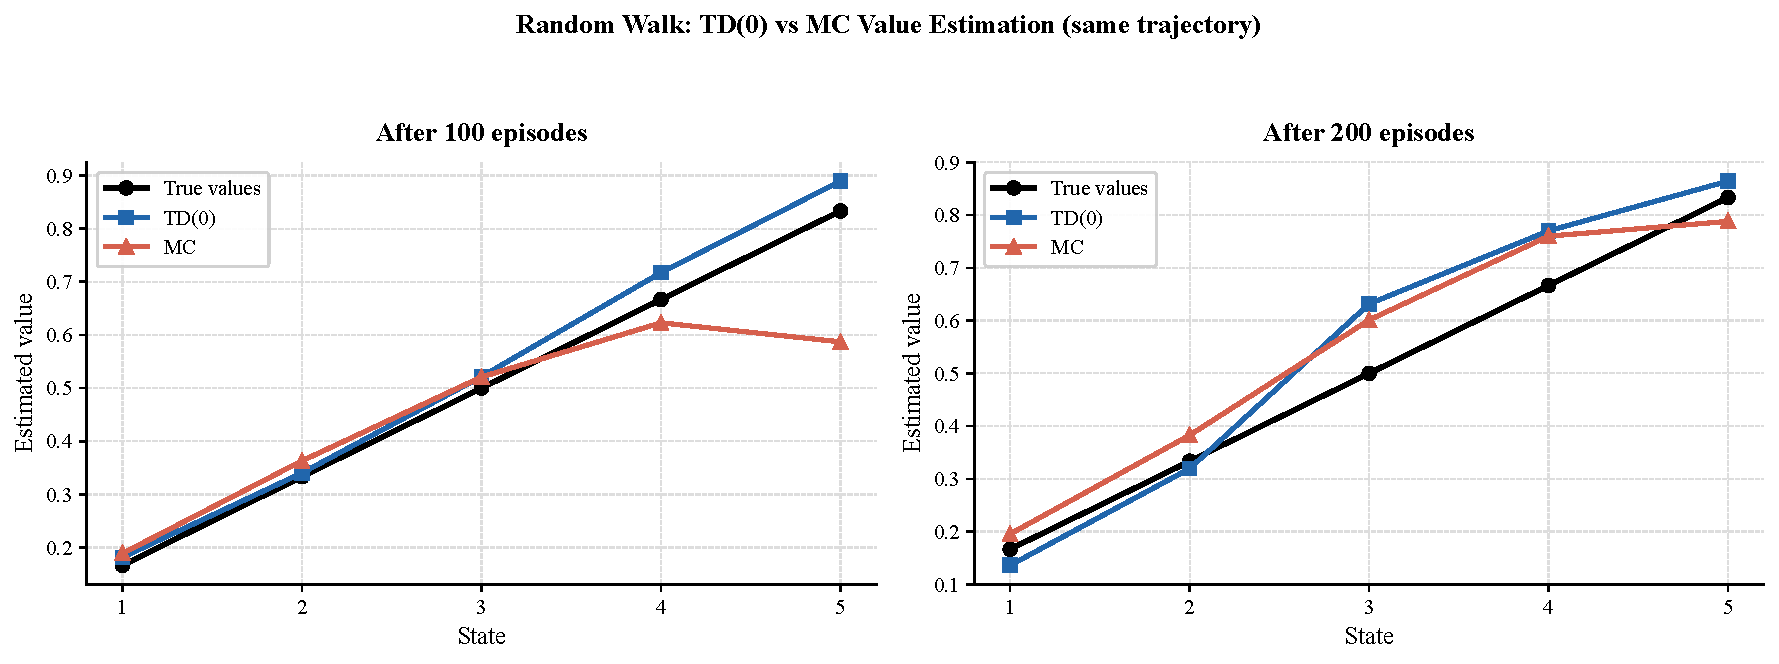
\includegraphics[width=0.85\textwidth]{fig1_random_walk_mc_vs_td.pdf}
  \caption{5 状态随机游走的价值估计（同一批轨迹）。黑线为真实价值 $v(s)=s/6$，红色为 MC（$\alpha=0.01$）、蓝色为 TD(0)（$\alpha=0.1$）。TD(0) 在 100、200 局后都更贴近真实值（100 局平均 RMS：MC 0.149 vs TD 0.062）。}
  \label{fig:td-vs-mc}
\end{figure}

% ============================================================
\section*{从预测到控制：SARSA 与 Q-Learning}

上一节用 $V$ 讲预测；本节用 $Q$ 讲控制（学策略）。

\subsection*{on-policy：SARSA}

SARSA 的目标是学习「当前实际执行的策略」（含探索）的 $q_\pi$：

\[
\boxed{Q(S_t,A_t) \leftarrow Q(S_t,A_t) + \alpha\bigl[R_{t+1} + \gamma Q(S_{t+1},A_{t+1}) - Q(S_t,A_t)\bigr]}
\]

动作选择通常用 $\varepsilon$-贪心。SARSA 的更新逻辑：
\begin{enumerate}
  \item 在 $S_t$ 按 $\varepsilon$-贪心选 $A_t$；
  \item 执行 $A_t$，得到 $R_{t+1}$，到达 $S_{t+1}$；
  \item 在 $S_{t+1}$ 按 $\varepsilon$-贪心\textbf{再选} $A_{t+1}$（不执行，只用它的 $Q$ 值）；
  \item 用 $A_{t+1}$ 的 $Q$ 值更新 $Q(S_t,A_t)$；
  \item $S_t \leftarrow S_{t+1}$，$A_t \leftarrow A_{t+1}$，重复。
\end{enumerate}

关键：目标中的 $A_{t+1}$ 来自\textbf{实际执行的策略}（含探索），因此 SARSA 学到的是 $\varepsilon$-贪心策略下的 $q_\pi$，\textbf{考虑到了探索的代价}。

\subsection*{off-policy：Q-Learning}

Q-Learning 学习\textbf{最优}（贪心）策略，但执行时仍用探索策略：

\[
\boxed{Q(S_t,A_t) \leftarrow Q(S_t,A_t) + \alpha\bigl[R_{t+1} + \gamma \max_a Q(S_{t+1},a) - Q(S_t,A_t)\bigr]}
\]

和 SARSA 的唯一区别：目标中用了 $\max_a Q(S_{t+1},a)$ 而不是 $Q(S_{t+1},A_{t+1})$。SARSA 的目标取决于实际选的动作 $A_{t+1}$（含探索噪音）；Q-Learning 的目标\textbf{总是假设下一步选最优动作}，无论实际探索做了什么。这就是 off-policy：\textbf{学习的策略}（贪心 = 最优）与\textbf{执行的策略}（$\varepsilon$-贪心 = 探索）不同。

\subsection*{SARSA vs Q-Learning：悬崖行走}

经典的 Cliff Walking 环境（$4\times12$ 格子，起点左下、目标右下，底部一行中间 10 格是悬崖：踩中回到起点并罚 $-100$，普通步罚 $-1$）揭示了两种算法的本质差异，如图~\ref{fig:cliff} 所示。

\begin{figure}[!htbp]
  \centering
  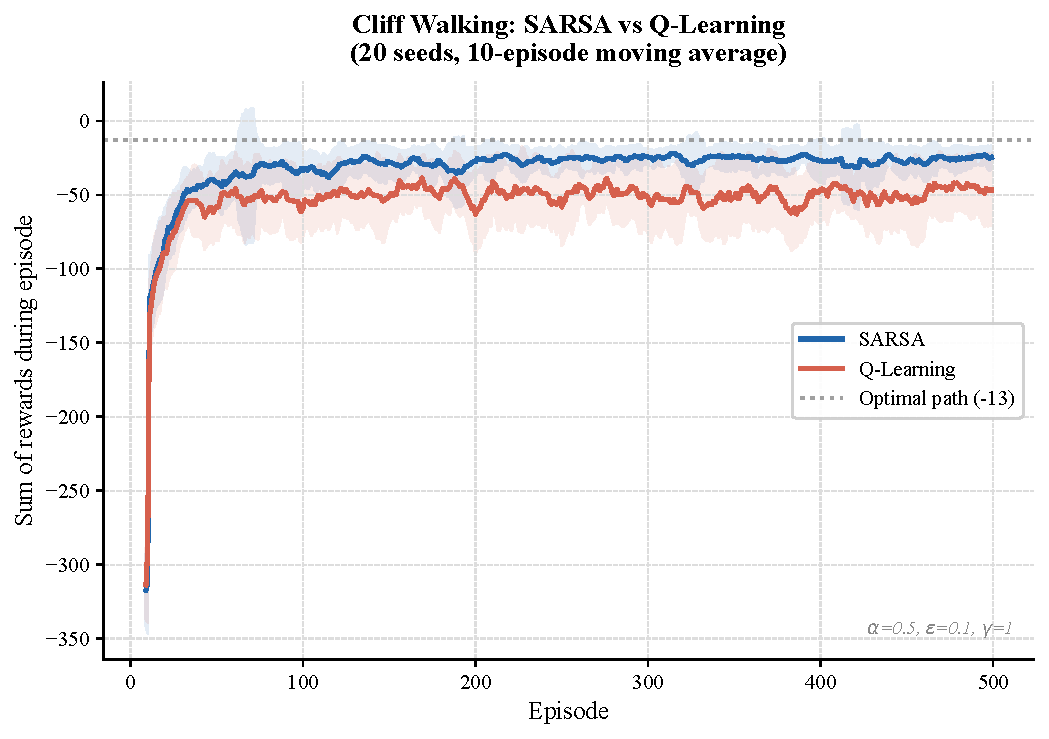
\includegraphics[width=0.85\textwidth]{fig3_cliff_sarsa_vs_qlearning.pdf}
  \caption{悬崖行走（$4\times12$，$\alpha=0.5$，$\varepsilon=0.1$，$\gamma=1$，20 个随机种子，10 局滑动平均）。训练期间 SARSA 的每局累计奖励显著高于 Q-Learning：SARSA 学到保守安全的绕行路线（偶尔探索也不至于灾难性坠崖），Q-Learning 学最短路径、但训练时因随机探索频繁坠崖。}
  \label{fig:cliff}
\end{figure}

\textbf{关键洞察}：Q-Learning 假设「下一步及以后都是最优的」，所以它认为贴崖走没问题（最优策略不会踩）；SARSA 知道实际执行时偶尔会探索，贴着悬崖走一次随机探索就是大灾难，因此学到更保守但安全的策略。如果部署时完全贪心（$\varepsilon=0$），Q-Learning 的激进策略可能更优——取决于你的 agent 在部署时还会不会犯错。

\subsection*{Expected SARSA 与 Softmax 策略}

\textbf{Expected SARSA} 不采样 $A_{t+1}$，而是对所有动作求期望，消除采样方差：

\[
Q(S_t,A_t) \leftarrow Q(S_t,A_t) + \alpha\Bigl[R_{t+1} + \gamma \sum_a \pi(a\mid S_{t+1})\,Q(S_{t+1},a) - Q(S_t,A_t)\Bigr]
\]

当目标策略 $\pi$ 是 $\varepsilon$-贪心时它是 on-policy；当 $\pi$ 是纯贪心时它\textbf{等价于 Q-Learning}（off-policy）。绝大多数任务上 Expected SARSA 优于传统 SARSA——微小的计算开销增加被方差下降带来的样本效率提升远远补偿。

\textbf{Softmax 策略}用温度 $\tau$ 按 $Q$ 值的相对大小分配探索概率：

\[
\pi(a\mid s) = \frac{\exp\bigl(Q(s,a)/\tau\bigr)}{\sum_b \exp\bigl(Q(s,b)/\tau\bigr)}
\]

$\tau$ 大趋于均匀探索，$\tau\to 0$ 趋于纯贪心。探索不再是盲目的（$\varepsilon$-贪心以 $\varepsilon$ 的概率随机探索，每个非贪心动作各以 $\varepsilon/|\mathcal{A}|$ 的概率被选中，包括明显差的），而是\textbf{更好的动作获得更多的选择概率}。

% ============================================================
\section*{多步扩展：N 步 TD 与 TD($\lambda$)}

\subsection*{N 步回报}

TD(0) 只看一步（低方差高偏差），MC 看全程（无偏高方差）。\textbf{N 步 TD} 是两者之间的连续谱，定义 $n$ 步回报：

\[
\boxed{G_t^{(n)} = R_{t+1} + \gamma R_{t+2} + \cdots + \gamma^{n-1}R_{t+n} + \gamma^n V(S_{t+n})}
\]

\begin{itemize}
  \item $n=1$：$G_t^{(1)} = R_{t+1}+\gamma V(S_{t+1})$ —— TD(0)；
  \item $n\to\infty$：$G_t^{(\infty)} = G_t$ —— MC；
  \item $1<n<\infty$：$n$ 个真实奖励 + 在第 $n$ 步截断处用 $V$ 估计余下部分。
\end{itemize}

更新式：$V(S_t) \leftarrow V(S_t) + \alpha\bigl[G_t^{(n)} - V(S_t)\bigr]$。N 步 SARSA 同理，只需把 $V$ 换成 $Q$，最后一项用 $\sum_a \pi(a\mid S_{t+n})Q(S_{t+n},a)$ 即为 Expected n-step SARSA。

图~\ref{fig:nstep} 展示了 $n$ 对偏差-方差权衡的影响：$n$ 越小（越依赖 bootstrapping）误差越低，$n$ 越大（越依赖真实奖励）越接近 MC 的高误差。

\begin{figure}[!htbp]
  \centering
  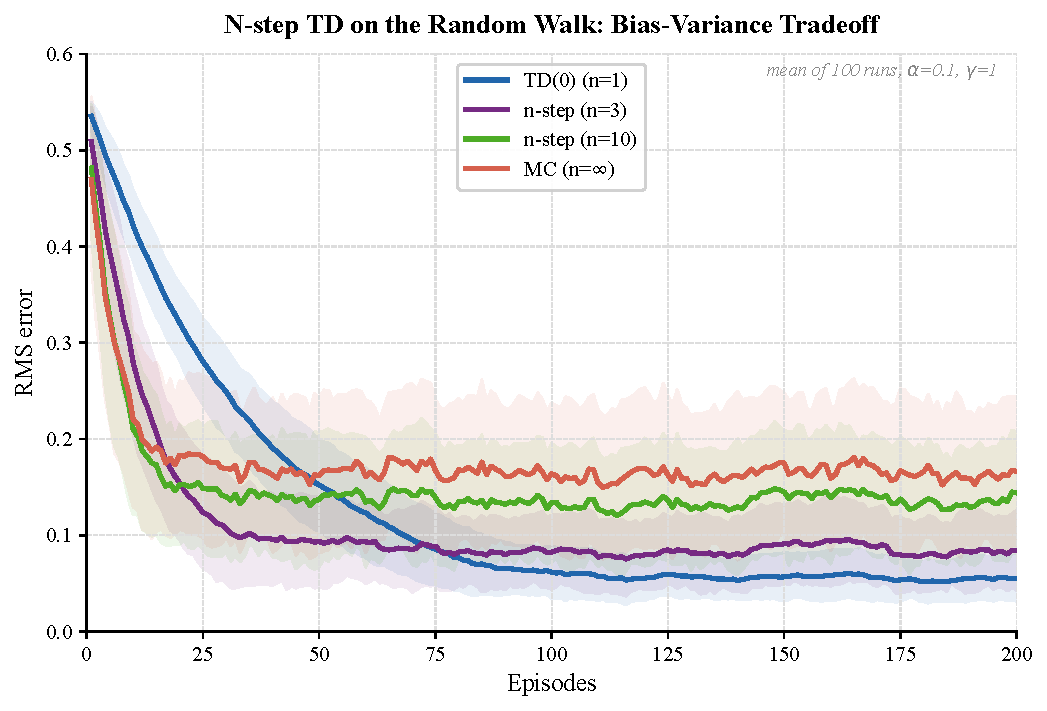
\includegraphics[width=0.85\textwidth]{fig2_nstep_bias_variance.pdf}
  \caption{5 状态随机游走上 N 步 TD 的 RMS 误差随局数的变化（同一 $\alpha=0.1$，平均 100 局）。$n=1$（TD(0)）误差最低，$n=3$、$n=10$ 依次上升，$n\to\infty$（MC）误差最高——$n$ 越小、bootstrap 越多，方差越小、学得越快。}
  \label{fig:nstep}
\end{figure}

\subsection*{TD($\lambda$)}

与其只用一个 $n$，TD($\lambda$) 把所有 $n$ 步回报用\textbf{几何加权平均}混合：

\[
\boxed{G_t^\lambda = (1-\lambda)\sum_{n=1}^{\infty} \lambda^{n-1} G_t^{(n)}}
\]

\begin{itemize}
  \item $\lambda=0$：$G_t^\lambda = G_t^{(1)}$ —— TD(0)；
  \item $\lambda=1$：$G_t^\lambda = G_t$ —— MC；
  \item $0<\lambda<1$：越近的步权重越大，越远的步贡献越小但非零。
\end{itemize}

$\lambda$ 控制 bootstrap 的程度：越小越依赖估计值（高偏差低方差），越大越依赖真实奖励（低偏差高方差）。

\subsection*{资格迹：TD($\lambda$) 的在线实现}

TD($\lambda$) 需要等到 episode 结束才能计算 $G_t^\lambda$（需要所有 $n$ 步回报）。\textbf{资格迹}（Eligibility Traces）提供在线增量式实现：每访问一个状态-动作对 $(s,a)$，给它的资格迹加 1，此后每步所有资格迹按 $\gamma\lambda$ 衰减：

\[
e_t(s,a) = \begin{cases}
  \gamma\lambda\, e_{t-1}(s,a) + 1, & \text{如果 } (s,a) \text{ 是当前对}, \\
  \gamma\lambda\, e_{t-1}(s,a),      & \text{否则}.
\end{cases}
\]

更新式：每一步对所有 $(s,a)$ 执行 $Q(s,a) \leftarrow Q(s,a) + \alpha\,\delta_t\, e(s,a)$。直觉：资格迹是「这个状态-动作对在多大程度上为当前结果负责」的衰减记录——越近的对权重越大，久远的对逐渐衰减归零。

\textbf{Watkins' Q($\lambda$)}：资格迹天然 on-policy，Q-Learning 是 off-policy 的，需要特殊处理——一旦执行了非贪心动作（探索），未来轨迹不再遵循目标策略，资格迹必须清零：

\[
\text{若 } A_{t+1} \neq \arg\max_a Q(S_{t+1},a) \;\Longrightarrow\; \text{所有 } e(s,a) \leftarrow 0
\]

代价：探索率高时，资格迹的有效长度取决于「连续贪心动作的长度」而非固定的 $\lambda$。

% ============================================================
\section*{经验回放——off-policy 的数据复用}

在线学习每步只用当前转移 $(S_t,A_t,R_{t+1},S_{t+1})$ 更新一次就丢弃，数据利用率极低。\textbf{经验回放}（Experience Replay）维护一个固定大小的缓冲，存储最近 $N$ 条转移：

\begin{enumerate}
  \item 执行策略产生新转移，存入缓冲；
  \item 从缓冲中\textbf{随机采样}一个 mini-batch；
  \item 在采样转移上做多次 Q-Learning 更新。
\end{enumerate}

为什么有效？
\begin{itemize}
  \item \textbf{打破相关性}：连续步的转移高度相关，随机采样打乱顺序，降低更新方差；
  \item \textbf{样本复用}：每条转移被多次使用，提高数据效率；
  \item \textbf{稳定训练}：相当于用了一组「旧数据」做正则化。
\end{itemize}

\textbf{限制}：经验回放只能用于 off-policy 算法（Q-Learning、Expected SARSA）。SARSA 不能用——它的更新依赖当前策略下的动作选择，而缓冲里的旧数据来自旧策略，不匹配。

% ============================================================
\section*{本章在 RL 体系中的位置}

\begin{enumerate}
  \item \textbf{上游}：MAB 的增量更新与探索-利用权衡、MDP 的 Bellman 方程与 DP 三种精确求解。DP 需要已知模型、MC 用真实回报（无偏高方差、需等回合结束），TD 取两者之长——一步采样 + bootstrap；
  \item \underline{\textbf{本章（TD 学习）}}：不依赖模型的价值学习核心——TD(0) 的一步更新、SARSA/Q-Learning 的 on/off-policy 分野、N 步与资格迹在偏差-方差之间调节、经验回放提升 off-policy 数据效率；
  \item \textbf{下游}：Q-Learning 的 $\max$ 算子 + 神经网络函数逼近 = DQN；经验回放 + 目标网络驯服 TD 更新的不稳定性（下一章）。
\end{enumerate}

\subsection*{TD 学习算法族谱}

\begin{center}
\begin{tabular}{lcccc}
\toprule
算法 & on/off-policy & Bootstrap & 目标形式 & 特点 \\
\midrule
MC & on & 否 & $G_t$ & 无偏，高方差 \\
TD(0) & on & 是 & $R+\gamma V(s')$ & 有偏，低方差 \\
SARSA & on & 是 & $R+\gamma Q(s',a')$ & 考虑探索代价 \\
Q-Learning & off & 是 & $R+\gamma\max_a Q(s',\cdot)$ & 学最优策略 \\
Expected SARSA & 均可 & 是 & $R+\gamma\sum_a\pi(a\mid s')Q(s',a)$ & 低方差 \\
N-step & 均可 & 是 & $n$ 步混合回报 & 偏差-方差可调 \\
Q($\lambda$) & off & 是 & $\lambda$-加权回报 + 资格迹 & 在线多步 \\
\bottomrule
\end{tabular}
\end{center}

\begin{itemize}
  \item \textbf{TD(0)}：一步真实奖励 + 下一步估计，无需等 episode 结束；
  \item \textbf{SARSA}：做什么就学什么，$\varepsilon$-贪心下的真实 $q_\pi$，保守安全；
  \item \textbf{Q-Learning}：直接学最优策略的 $q_*$，不管实际如何探索；
  \item \textbf{Expected SARSA}：对采样求平均，降低方差，可退化为 Q-Learning；
  \item \textbf{N-step TD}：折中偏差和方差，越大的 $n$ 越接近 MC；
  \item \textbf{TD($\lambda$) + 资格迹}：用指数衰减对每步误差分配功劳，在线实现多步传播；
  \item \textbf{经验回放}：存旧数据、随机重放，打破相关性、提升样本效率（仅 off-policy 可用）。
\end{itemize}

\subsection*{从 TD 到 DQN 的桥梁}

\begin{enumerate}
  \item \textbf{Q-Learning 的 $\max$ 算子 + 函数逼近} = DQN（Deep Q-Network）；
  \item \textbf{经验回放 + 目标网络} = 解决 DQN 中 TD 更新的不稳定性；
  \item $\varepsilon$-\textbf{贪心探索}被延续到 DQN 中（简单但有效，后来被 NoisyNet 等方法改进）；
  \item \textbf{资格迹}的思想 $\to$ Retrace 算法 $\to$ 结合经验回放实现高效 off-policy 多步学习。
\end{enumerate}

学完本章，你掌握了「不依赖模型」的价值学习核心——TD 用 bootstrapping 换方差、SARSA/Q-Learning 区分 on/off-policy、N 步与资格迹在偏差-方差之间调节。下一章 DQN 把 Q-Learning 的表格换成神经网络，并用经验回放与目标网络驯服它的不稳定性。

\subsection*{参考资料}

\begin{enumerate}
  \item Sutton \& Barto (2018). \textit{Reinforcement Learning: An Introduction} (2nd ed.). Chapters 6--7, 12.
  \item Watkins, C.\ J.\ C.\ H. (1989). \textit{Learning from Delayed Rewards}. PhD Thesis.（Q-Learning 原始论文）
  \item Rummery \& Niranjan (1994). On-line Q-learning using connectionist systems.（SARSA 原始论文）
  \item van Seijen et al. (2009). A theoretical and empirical analysis of Expected Sarsa.
  \item Lin (1992). Self-improving reactive agents based on reinforcement learning.（Experience Replay 的发明）
  \item Mnih et al. (2015). Human-level control through deep reinforcement learning. \textit{Nature}.（DQN + Experience Replay）
  \item Practical RL, Yandex Data School. Week 3——Model-Free Reinforcement Learning.
\end{enumerate}

\end{document}
